\appendix
\section{Risks, Limitations and Ethical Considerations}
\label{sec:risks_challenges}
% Alongside these opportunities, risks and challenges must be addressed.
\subsection*{Risk}
Over-reliance on LLMs without rigorous verification could embed subtle errors into research~\cite{Zhang2023Sirens}. The potential for LLMs to ``cheat'' reward functions during fine-tuning, producing plausible but physically invalid outputs (e.g., a simulation appearing to conserve energy due to numerical artifacts), requires careful alignment and robust evaluation~\cite{Bengio2024Managing,Anwar2024Foundational}.
Furthermore, depending too heavily on LLMs for tasks like mathematical derivations (e.g., routinely asking an LLM to compute integrals like $\int d^4k / (k^2-m^2+i\epsilon)^2$ instead of learning contour integration techniques), programming, or data interpretation could risk degrading these essential skills among physicists, especially those in training~\cite{Bender2020Climbing}. Deep intuition often arises from performing detailed calculations firsthand.
% Overreliance on LLMs for these steps might trade this deeper understanding for superficial ease~\cite{TaoBlogOnAI}.
% Maintaining critical thinking, independent problem-solving abilities, and verification skills remains necessary even as LLM capabilities advance.
The history of scientific computing shows both warnings and reassurances: tools like Mathematica initially raised de-skilling concerns but ultimately enabled mathematicians to focus on higher-level work by automating repetitive calculations. Similarly, LLMs could potentially elevate physics research by handling routine tasks while humans focus on deeper insights---if used as augmentation rather than replacement for fundamental understanding.

\subsection*{Limitations}
\label{sec:limitations}
This position paper presents a high-level overview. The field of LLMs is rapidly evolving, and specific capabilities or limitations discussed may change quickly.
Due to the rapid evolution of LLMs, specific examples quickly become outdated. The selected examples are illustrative of general trends observed circa late 2024 and early 2025. The scope is necessarily limited to selected aspects of physics research, and specific examples may not generalize to all subfields.
\subsection*{Ethical Considerations}
\label{sec:ethics}
Generating plausible but incorrect claims requires rigorous validation. Training bias could steer research suboptimally. Responsible deployment and human oversight are required. Access and equity issues must be addressed to ensure broad availability of these tools across the global physics community.

\section{Related Works}
\paragraph{Non-Language Models Already Help Physics}
Machine learning (ML) is not new to physics~\cite{Carleo2019Machine}. Current applications include analyzing large experimental datasets (e.g., particle identification at the Large Hadron Collider~\cite{Guest2018Deep}), solving computational physics problems (e.g., finding ground states of quantum Hamiltonians like $H\psi = E\psi$~\cite{Carleo2017Solving,Glasser2018NeuralNetwork}), accelerating partial differential equation solvers~\cite{Karniadakis2021Physicsinformed}, and optimizing experimental controls (e.g., plasma shaping in fusion reactors~\cite{Degrave2022Magnetic}).
These applications typically involve supervised learning (classification, regression), unsupervised learning (clustering, dimensionality reduction, generative modeling), or reinforcement learning for specific, well-defined tasks. While powerful for specific tasks, these methods often differ from the requirements of open-ended theoretical exploration, complex multistep problem solving, or nuanced experimental design where LLMs might offer complementary advantages through their natural language interface and broad knowledge encoding~\cite{Schaeffer2023Are,Lewkowycz2022Solving}.
\section{More Examples}
\paragraph{Example: Notational Nuances}
Another example is the Bogoliubov-de Gennes (BdG) Hamiltonian, which often includes a $1/2$ prefactor by convention; LLMs might add or omit this factor inconsistently if not carefully prompted, thereby impacting all subsequent calculations even though the authors intend a different factor.
\paragraph{Example: Lattice Gauge Theory}
For example, implementing the pure gauge SU(2) Hamiltonian:
\begin{equation}
    H = \frac{g^2}{2} \sum_l \hat{E}^a_l \hat{E}^a_l + \frac{1}{2g^2} \sum_p \left(2 - \text{Tr}(\hat{U}_p + \hat{U}_p^\dagger)\right)
\end{equation}
where $\hat{E}^a_l$ are electric field operators on links $l$, $\hat{U}_p$ are plaquette operators, and $g$ is the coupling constant, requires translating abstract gauge theory concepts into concrete numerical algorithms that preserve gauge invariance and other symmetries.
A critical physical constraint in such simulations is ensuring that states satisfy Gauss's law, which in the quantum context becomes $\sum_{l \in \text{star}(n)} \hat{E}^a_l |\psi\rangle_{\text{phys}} = 0$ for each lattice site $n$ and each gauge group generator $a$. This constraint must be explicitly enforced in the code, typically by projecting onto the physical subspace or by adding an energy penalty term.

\paragraph{Example: Explaining the derivations}
A research paper may state a key result derived from an effective action, $S_{\text{eff}}[\phi_c]$, obtained by ``integrating out'' high-momentum modes $\phi_h$ from a full action $S[\phi_c, \phi_h]$. An LLM assisting a researcher could be tasked to elaborate on the formal path integral definition $e^{-S_{\text{eff}}[\phi_c]/\hbar} = \int \mathcal{D}\phi_h e^{-S[\phi_c, \phi_h]/\hbar}$. This elaboration might involve expanding the derivations with common evaluation techniques like saddle-point approximations or perturbative expansions of $S[\phi_c, \phi_h]$ around a background field, all while strictly adhering to the paper's specific notation for the classical fields $\phi_c$ and quantum fluctuations $\phi_h$.

\paragraph{Example: Diagonalizing a 2x2 Hermitian matrix}
When asked to diagonalize a general 2x2 Hermitian matrix $H = \begin{pmatrix} a & b-ic \\ b+ic & d \end{pmatrix}$ (where $a,b,c,d$ are real but have complex expressions), an LLM might default to a brute-force symbolic expansion of the characteristic determinant $\det(H - \lambda I) = 0$ to find eigenvalues, followed by solving systems of linear equations for eigenvectors. A `good AI physicist', however, might recognize the structure and suggest decomposing the matrix in the Pauli basis: $H = a_0 I + \mathbf{a} \cdot \boldsymbol{\sigma}$, where $I$ is the identity matrix, $\boldsymbol{\sigma} = (\sigma_x, \sigma_y, \sigma_z)$ are the Pauli matrices, $a_0 = (a+d)/2$, and $\mathbf{a} = (b, c, (a-d)/2)$. From this decomposition, eigenvalues ($a_0 \pm |\mathbf{a}|$) and eigenvectors (related to the direction of $\mathbf{a}$) can be read off with greater physical insight (e.g., connecting to spin precession in a magnetic field) and often less computation. Training LLMs to prefer such insightful decompositions over brute-force methods is key to developing AI assistants that contribute to more elegant theory and can reduce complex algebraic manipulations where errors might occur.

\paragraph{Example: Feynman diagram}
Interpreting a Feynman diagram~\cite{Feynman1949Theory} for Compton scattering ($\gamma e^- \to \gamma e^-$) (see, e.g.,~\cite{Peskin1995Introduction}) requires identifying incoming/outgoing photon (wavy lines) and electron (solid lines) lines, internal propagators (e.g., electron propagator $S_F(p) = i(\gamma \cdot p + m_e)/(p^2-m_e^2+i\epsilon)$, where $m_e$ is electron mass, $e$ is elementary charge, $\gamma^\mu$ are Dirac gamma matrices), and vertices (e.g., QED vertex factor $-ie\gamma^\mu$). An LLM should connect these diagrammatic elements to the mathematical terms in the scattering amplitude calculation according to Feynman rules.
\begin{figure}[h!]
    \centering
    % \begin{tikzpicture}
    % \begin{feynman}
    % \diagram[horizontal=a to b] {
    % i1 [particle=$e^{-}$] -- [fermion,momentum'=$p_{i}$] a -- [photon,reversed momentum'=$k_{i}$] f1 [particle=$\gamma$],
    % a -- [fermion] b,
    % i2 [particle=$\gamma$] -- [photon,reversed momentum'=$k_{f}$] b -- [fermion,momentum'=$p_{f}$] f2 [particle=$e^{-}$],
    % };
    % \end{feynman}
    % \end{tikzpicture}
    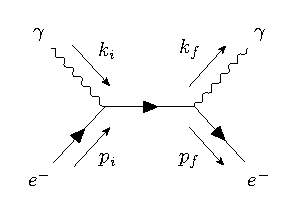
\includegraphics[width=0.45\textwidth]{Sections/feynman_diagram_example.pdf}
    \caption{A Feynman diagram for Compton scattering ($\gamma e^- \to \gamma e^-$) in s-channel. LLMs should connect graphical elements (straight lines for fermions, wavy lines for bosons, and vertices for interactions) to mathematical terms in scattering amplitude calculations (e.g., propagators, vertex factors, external leg factors).}
    \label{fig:feynman_diagram_example}
\end{figure}

\paragraph{Example: Physical Inaccuracy in AI-Generated Images}
Current AI image generators lack physical understanding, producing visually appealing but scientifically incorrect visualizations. Figure~\ref{fig:peps_ai_generated} shows GPT-4o's response to ``generate an image of a 3D modeling of a two dimensional projected entangled pair state tensor network (4 by 4 square lattice)''. The image violates PEPS structure: bulk tensors require exactly five indices (four virtual bonds to neighbors, one physical index), yet many nodes show incorrect connectivity. AI systems fail to encode the physical constraints---here, tensor network geometry and index structure.
\begin{figure}[h]
    \centering
    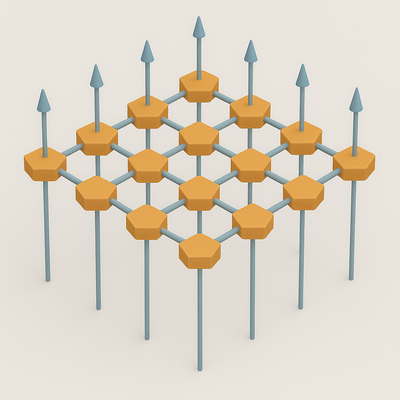
\includegraphics[width=0.5\textwidth]{Sections/PEPS_paper.png}
    \caption{GPT-4o-generated PEPS network with incorrect or at least unconventional tensor connectivity. Proper PEPS tensors need 5 indices (4 virtual, 1 physical); many nodes lack required connections.}
    \label{fig:peps_ai_generated}
\end{figure}

\paragraph{Example: AI Material Physicist}
Imagine a physicist investigating a novel topological material. An `AI Physicist' assistant might: (1) Synthesize recent literature on related materials and their Berry curvature $\Omega_{n,xy}(\mathbf{k})$ calculations. (2) Assist in formulating a tight-binding Hamiltonian $H(\mathbf{k})$ for the new material based on its crystal structure (e.g., honeycomb lattice for graphene-like systems). (3) Generate Python code using libraries like Kwant or TightBindingTools.jl to numerically calculate the band structure $E_n(\mathbf{k})$ and Chern numbers $C_n = \frac{1}{2\pi} \int_{BZ} d^2k \Omega_{n,xy}(\mathbf{k})$. (4) If numerical results show unexpected edge states, it might help consider analytical approximations (e.g., a low-energy effective Dirac Hamiltonian $H_{eff} = v_F (k_x \sigma_y - k_y \sigma_x) + m \sigma_z$, where $v_F$ is the Fermi velocity and $m$ is a mass/gap parameter) to understand their origin. (5) Finally, it might create a slide deck summarizing these findings, including generating plots. This collaborative workflow, with the AI handling complex but definable subtasks under human strategic guidance, shows the potential~\cite{Wang2023Scientific}.

\paragraph{Example: Verifying analytical calculations by Mathematica}
Consider the Jordan-Wigner transformation, useful for 1D quantum spin systems. The transverse field Ising model Hamiltonian is $H = -J \sum_{\langle i,j \rangle} \sigma_i^z \sigma_j^z - h \sum_i \sigma_i^x$. The transformation maps spin operators $\sigma_i^\alpha$ to fermionic operators $c_j, c_j^\dagger$, e.g., $\sigma_j^z = 2c_j^\dagger c_j - 1$ and $\sigma_j^x = (\prod_{k<j} (1-2c_k^\dagger c_k)) (c_j + c_j^\dagger)$. An LLM might attempt this transformation and could be asked to verify parts via a Mathematica MCP, such as the anticommutation relation of the fermionic operators after the transformation $\{c_j, c_j^\dagger\}$. Using symbolic tools such as Mathematica, the probability of correctness can be increased, if LLMs become better at generating the correct query for a tool and interpreting its output for such (and more nontrivial) operator algebra.


\section{More Analysis}

\subsection{Building Better UI/UX for Human-centered AI}
\label{sec:building_better_ui_ux}
For LLMs to be effective collaborators, intuitive and efficient user interfaces (UIs) and user experiences (UXs) are essential for supervision, tracing, and trust-building. These interfaces should allow physicists to interact with LLMs naturally without extensive prompt engineering and should integrate with existing research workflows and tools (e.g., LaTeX editors, data analysis and simulation environments).
Future LLMs should also be robust to specific prompts and offer finer-grained controllability over their reasoning style, level of detail, and assumptions made. For instance, prompting an LLM to ``solve the Schr{\"o}dinger equation for a particle in a box'' might yield different solution forms depending on subtle phrasing. Ideally, an LLM should recognize standard conventions (e.g., specific boundary conditions $\psi(0)=\psi(L)=0$ for a box of length $L$) or prompt for these if ambiguous. Controllability would allow a physicist to specify, for example, ``provide a solution using separation of variables and show all steps for $H\psi = E\psi$ where $H = -\hbar^2/2m \cdot d^2/dx^2 + V(x)$ and $V(x)=0$ for $0<x<L$, $\infty$ otherwise'' versus ``give the energy eigenvalues $E_n = \frac{n^2\pi^2\hbar^2}{2mL^2}$ and normalized wavefunctions $\psi_n(x) = \sqrt{2/L}\sin(n\pi x/L)$ directly''. Such controllability is vital for making LLMs reliable and adaptive research assistants.
Effective UI/UX must go beyond simple chat interfaces. Physicists often work with extensive comments, annotations, and margin notes; interfaces supporting these natural workflows would be more effective. For supervising agents, UIs need robust mechanisms for managing experimental/simulation results, tracking context across long interactions (context management~\cite{Sumers2023Cognitive}), and accommodating human-in-the-loop intervention. Given that LLM outputs can be verbose, tools for generating structured summaries with highlighting are needed. Integration with collaborative platforms (e.g., Overleaf-like features with LLM assistance for consistency checking in \LaTeX{} documents, or GitHub-style review tools for coding and derivations) would also be convenient.
% Lowering the barrier for prompting through automated frameworks~\cite{Shin2020AutoPrompt,Reynolds2021Prompt} or structured approaches like DSPy~\cite{Khattab2023DSPy} could also be helpful for widespread adoption, though the complexity of such advanced prompting systems must be managed.

\subsection{Running Physical Experiments}
\label{sec:future:inter_ctrl_exp}
While our primary focus is on theoretical physics, we acknowledge that in the long term, AI systems might also actively control experimental instrumentation, interpret sensory data in real-time, and adjust experimental parameters accordingly. This would require the seamless integration of perception (e.g., using computer vision to optimize laser beam path setup for quantum optics experiments where alignment precision is critical for data quality), reasoning (understanding the experimental progress and deciding which measurements to perform next based on acquired data), and action (subsequently adjusting the lensing setup with high-precision robotic arms) in the physical world. This long-term vision enables a dynamic integration of reasoning models with robotics and control theory, bridging high-level human-defined agenda with corresponding physical actions as envisioned by rising interest in Large Action Models (LAM)~\cite{Wang2025Large} and Embodied Intelligence~\cite{Liu2025Embodied}.